%\documentclass[12pt,xcolor=dvipsnames,mathserif]{beamer}
\documentclass[12pt,xcolor=dvipsnames,handout,mathserif,aspectratio=169]{beamer}

\usepackage{hyperref}

\usepackage{pgfpages}
\usepackage{colortbl}
\usepackage{multirow}

%\pgfpagesuselayout{2 on 1}[border shrink=2.5mm]
%\pgfpageslogicalpageoptions{1}{border code=\pgfusepath{stroke}}
%\pgfpageslogicalpageoptions{2}{border code=\pgfusepath{stroke}}


% Specify theme
%\usetheme{Madrid}
\usetheme{Boadilla}
% See deic.uab.es/~iblanes/beamer_gallery/index_by_theme.html for other themes

% Specify base color
%\usecolortheme[named=OliveGreen]{structure}
\usecolortheme[named=RoyalBlue]{structure}
% See http://goo.gl/p0Phn for other colors

% Specify other colors and options as required
\setbeamercolor{alerted text}{fg=Red}
\setbeamertemplate{items}[square]

% Specify some useful short commands
\newcommand{\bbl}[1]{{\color{NavyBlue} \textbf{#1}}}
\newcommand{\bre}[1]{{\color{red} \textbf{#1}}}
\newcommand{\bgr}[1]{{\color{PineGreen} \textbf{#1}}}
\newcommand{\un}{\texttt{\char`_}}
\newcommand{\tcb}{\textcolor{blue}}


% Title and author information
\title[Introductory Statistics with Excel]{Introductory Statistics with Excel}
\author[Andrew Parnell]{Andrew Parnell}
\institute[UCD]{University College Dublin \begin{center} \includegraphics[width=1.5cm]{UCDlogo.pdf}\end{center} }
\date[Class 3]{Class 3 - Hypothesis testing}
%\date{Lecture 2 -- part 1}

\begin{document}

\titlepage

\begin{frame}{Learning outcomes}

In this class we will cover
\begin{itemize}
\item Sampling distributions
\item Setting up hypothesis test
\item The working of a hypothesis test
\item Interpreting the output of a hypothesis test
\end{itemize}

\end{frame}

\begin{frame}{Statistical inference and sampling distributions}

Why are we doing statistical inference? Consider the following examples:
\begin{itemize}
\item We have a new drug which might be used to treat those suffering with cancer. We trial the drug in an RCT. How do we know whether the drug works or not?
\pause
\item The mean northern hemisphere temperature has risen from around 13$^\circ$C (1980-1990 average) to around 19$^\circ$C (2000-2010 average). How do we know this difference is real and not just from random chance? 
\pause
\item A new particle, purported to be the Higgs Boson, has been found at mass 125GeV after an experiment at CERN. How do we know whether this particle is really there or whether it was just experimental chance?
\end{itemize}


\end{frame}

\begin{frame}{Parameters}

\begin{block}{Reminder}
We are interested in estimating \bre{parameters}: characteristics of interest from the \bgr{population}. We assume that the parameter is an unchanging, fixed value
\end{block}
\pause
\vspace{0.2cm}
Examples of parameters:
\begin{itemize}
\item The proportion of the population that consider themselves left-handed
\item The probability that a baby who sleeps with a night light suffers from myopia at age 20
\item The income difference between arable and pastural farmers
\end{itemize}
\end{frame}

\begin{frame}{Statistics}

\begin{block}{Reminder}
A \bbl{statistic} is an estimate computed from a sample of data. These data may have been collected from a trial, an experiment, an observational study, or a survey. We often try to choose statistics that are \bgr{good estimators} of the parameters
\end{block}
\pause
Examples of statistics:
\begin{itemize}
\item The sample proportion of 100 people who consider themselves left-handed
\item The sample proportion of adults aged 20 with myopia from a sample of adults aged 20 who had night lights as babies
\item The sample mean income difference between arable and pastural farmers
\end{itemize}
\end{frame}

\begin{frame}{Key ideas}

\begin{block}{}
\begin{itemize}
\item These statistics are just \bre{estimates} of the parameters. If we ran the experiment again we would get different values of the statistics. These estimators are \bre{uncertain} and the statistics are \bbl{random variables}
\item If we can make some assumptions about the behaviour of the statistic over different samples we can create the \bgr{sampling distribution} of the statistic
\item The practice of estimating parameters from statistics taking into account their uncertainty is called \bbl{statistical inference}
\item We will cover two parts of statistical inference: \bgr{confidence intervals} and \bre{hypothesis testing}
\end{itemize}
\end{block}

\end{frame}


\begin{frame}{Answering questions about parameters}

One of the great things about statistics (and maths in general) is that the \bre{methods} used in all sorts of different applications turn out to be the same. However, it can be quite difficult to translate from the questions of scientific interest into questions about parameters which are amenable to statistical analysis.
\pause
\begin{block}{Example}
Do pigs on fodder produce higher quality meat than those who forage? Possible parameters of interest: 
\begin{itemize}
\item proportion of pigs on fodder with higher quality meat than those who forage
\item average meat quality increase between fodder/foraging pigs
\end{itemize}
\pause
We could then run a study of pigs measuring their meat quality on each of the different feed types
\end{block}

\end{frame}

\begin{frame}[fragile]{}
\bbl{\Huge Sampling distributions of statistics}\\ 
\vspace{0.5cm}
\end{frame}

\begin{frame}{Statistics as random variables}

\begin{block}{Important}
We can think of taking a sample or conducting an experiment as one big random circumstance. The value of the statistic is then one possible outcome of that random circumstance. Thus a statistic is just a \bre{random variable} and has an associated \bbl{probability distribution} (or probability density). We call the probability distribution of a statistic the \bgr{sampling distribution}
\end{block}
\pause
\vspace{0.2cm}
If we know the probability distribution then we can make statements about the parameter from the probability distribution. We can then work out, for example, the probability that the statistic lies in the range $(a,b)$ or the probability that the statistic is bigger than a chosen value.
\end{frame}

\begin{frame}{Features of sampling distributions}

In the situations we will cover:
\begin{itemize}
\item The sampling distribution is \bbl{approximately normal}. Remarkably this occurs all the time (see associated app -- \url{https://gallery.shinyapps.io/CLT_mean/}).
\item The mean of the sampling distribution is the \bre{value of the parameter}. For example, the mean of the sampling distribution for the sample mean is the true parameter value
\item The standard deviation of the sampling distribution measures how the value of the statistics \bre{vary} over across different samples
\end{itemize}
\pause
Remember that the normal distribution is \bgr{completely defined} by its mean and standard deviation (or variance). So to specify the sampling distribution we only need to calculate the mean and the standard deviation

\end{frame}

\begin{frame}{Standard error}

\begin{block}{Definition}
The sample standard deviation for a statistic is known as the \bre{standard error}.
\end{block}
\vspace{0.5cm}
\pause
Note that this is different to the standard deviation of the data (again see app). To be clear, we append the name of the statistic on to the end of the name, so that the standard deviation of the sample mean is written as the \bbl{standard error of the mean}
\end{frame}

\begin{frame}[fragile]{}
\bbl{\Huge Hypothesis tests}\\ 
\vspace{0.5cm}
\end{frame}

\begin{frame}\frametitle{Example}
Reminder of the milk yield data: \\
\vspace{0.5cm}
\begin{tabular}{ccccccc}
169.6&142&103.3&111.6&123.4&143.5&155.1\\
101.7&170.7&113.2&130.9&146.1&169.3&155.5
\end{tabular}
\vspace{0.5cm}

\begin{enumerate}
\item Want to investigate the farmer's claim that the mean weekly milk yield for the herd is 120kg.
\vspace{0.2cm}
\item What error could the we make when making their decision?
\vspace{0.2cm}
\item Want to assess uncertainty in mean weekly milk yield -- construct and interpret a 95\% confidence interval for the mean milk yield.
\end{enumerate}

\end{frame}

\begin{frame}
\frametitle{Hypothesis Testing}
Hypothesis testing involves two contradictory hypotheses:
\begin{itemize}
\item The Null Hypothesis ($H_0$), initially assumed to be true.
\item The Alternative Hypothesis ($H_A$).
\end{itemize}
$\:$\\
These hypotheses are equivalent to the innocent ($H_0$) until proven guilty ($H_A$) in a court of law. \\
\vspace*{0.4cm}
We examine the evidence (the \bbl{data}) to see if it proves guilt; we do not try to prove innocence as the defendant is presumed innocent until proven guilty. \\
\vspace*{0.4cm}
Hence, when we choose the hypotheses, $H_A$ should be the hypothesis for which we seek evidence.\\
\vspace*{0.4cm}
NOTE: The same hypothesised value must be used in $H_A$ as in $H_0$.
\end{frame}


\begin{frame}
\frametitle{Hypothesis Testing}
The decision whether or not to reject $H_0$ is based on the evidence contained in the sample \bbl{data}.\\
\vspace*{0.5cm}
The result of the hypothesis test will be either:
\begin{itemize}
\item Reject $H_0$ in favour of $H_A$: when the data provide sufficient evidence that $H_A$ is true. The result is said to be \bbl{statistically significant}.
\vspace{0.5cm}
\item Fail to reject $H_0$: when we have insufficient evidence that $H_A$ is true. The result is not \bbl{statistically significant}.
\end{itemize}
\vspace{0.5cm}
\pause
\bbl{Note:} Failing to reject $H_0$ does not mean that we have evidence that it is true - we simply do not have sufficient evidence to reject it. Failing to prove guilt does not prove innocence!!
\end{frame}

\begin{frame}
\frametitle{Incorrect Decisions}
\vspace*{0.5cm}
\begin{center}{\large{
\begin{tabular}{|l|cc|} \hline
& \multicolumn{2}{|c|}{\bbl{The Truth}}\\ \hline
\bbl{The Decision}&$H_0$ True & $H_A$ True\\ \hline
Reject $H_0$&Type I error& :)\\
Do not reject $H_0$&:)&Type II error\\ \hline
\end{tabular}}}\end{center}

Type I error: Reject the Null Hypothesis when it is true.
Type II errors: Do not reject the Null Hypothesis when it is false.
\pause

\vspace*{0.5cm}
\bbl{LEGAL ANALOGY:}

\vspace*{0.2cm}
$H_0$: Innocent  and  $H_A$: Guilty

\vspace*{0.3cm}
Type I error: Innocent person found guilty.

\vspace*{0.3cm}
Type II error: Guilty person found innocent.
\end{frame}


\begin{frame}
\frametitle{Incorrect Decisions}
The advantage of using statistical hypothesis testing instead of any other decision making procedure is that we can quantify and control the probability of making a type I or type II error.

\vspace*{0.5cm}
The Probability of a \bbl{Type 1} error is called the \bgr{significance level} of the test.\\
The Probability of a \bbl{Type 2} error is one minus the \bre{power} of the test.\\

\vspace*{0.5cm}
Reducing the significance level increases the power and vice versa. The only way to improve both is to increase the sample size.

\vspace*{0.5cm}
The value of the significance level is decided by the statistician and the values usually used are 0.05 or 0.01.\\
\vspace*{0.5cm}
(These values have statistical motivation -- they're not just randomly chosen values!)
\end{frame}

\begin{frame}{Power and significance}

\centering \includegraphics[width=0.7\textwidth]{Power.pdf}

\tiny
Taken from \url{https://qph.ec.quoracdn.net/}
\end{frame}


\begin{frame}\frametitle{Test Statistics and Rejection Regions}
Assuming $H_0$ is true, we compute a \bbl{test statistic} which follows a known distribution (e.g. the Normal distribution).\\
$$\mbox{\bbl{test statistic}} = \frac{\mbox{sample statistic - null value}}{\mbox{standard error}} $$

\vspace{0.5cm}
When we have a large sample (n$\geq$30) the Central Limit Theorem
tells us that, irrespective of the underlying population distribution, a mean has approximately a \bbl{Normal} distribution with:
\vspace*{0.5cm}
\begin{itemize}
\item mean $ = $ population mean (the value in $H_0$).\\
\item standard error $=$ $\mbox{sample standard deviation} / \sqrt{n}$. \\(the \bbl{standard error} - see earlier app)\\
\end{itemize}
\end{frame}

\begin{frame}
\frametitle{Test Statistics and Rejection Regions}
Hence, our test statistic
$$\frac{\mbox{sample statistic - null value}}{\mbox{standard error}}$$
has a \bbl{standard Normal} distribution (i.e. mean 0 and standard deviation 1).\\
\centering 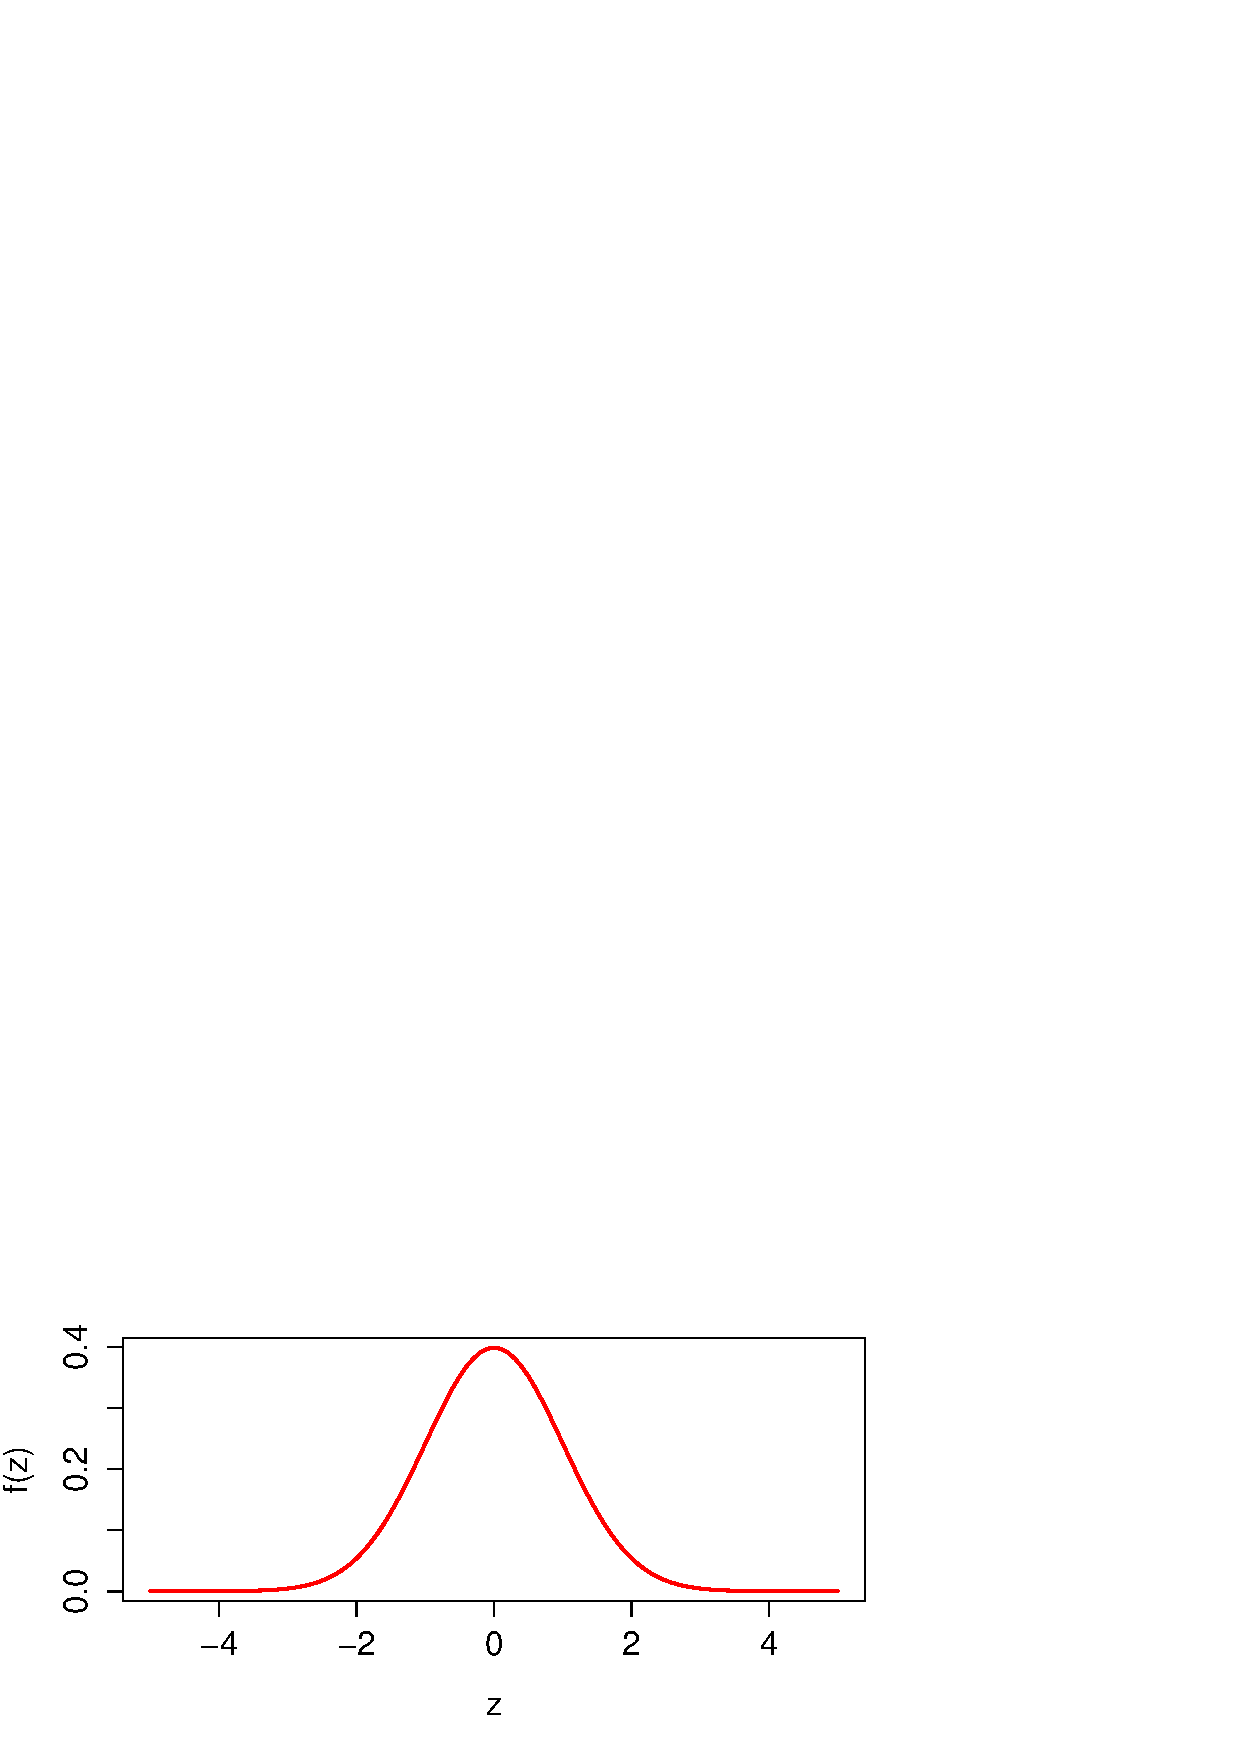
\includegraphics[width=0.5\textwidth]{NormalPDF.pdf}
\end{frame}

\begin{frame}
\frametitle{Test Statistics and Rejection Regions}
The \bbl{critical value(s)} divide the possible values of the test statistic into a \bbl{rejection region} and a \bbl{nonrejection region}.\\
\vspace*{0.5cm}
The critical values depend on the significance level of the test $\alpha$.\\
\vspace*{0.5cm}
Why?
\begin{itemize}
\item If $H_0$ is true, the sample statistic is unlikely to be very different from the hypothesized value.\\
\item Or, a test statistic very different from 0 is unlikely.\\
\item The significance level is the value we assign to the word `unlikely'.\\
\item If the test statistic lies in the rejection region we reject $H_0$ as the probability it lies there is below
what we defined as `unlikely'.\\
\end{itemize}
\end{frame}

\begin{frame}{Back to the cows data}

\begin{itemize}
\item We want to test whether the mean value is 120 or not so $H_0$: population mean = 120, vs $H_A$: population mean $\ne 120$.\\
\item We already know the sample mean is 138.3kg and the sample standard deviation is 24.6kg
\item We have 14 observations so that standard error of the mean is $\frac{24.6}{\sqrt{14}} = 6.56$.\\
\item Our test-statistic is then: $\frac{\mbox{sample statistic - null value}}{\mbox{standard error}} = \frac{138.3 - 120}{6.56} = 2.78.$
\item The 97.5th percentile of the standard normal distribution is 1.96 (Excel - \texttt{NORM.INV(0.975,0,1)}). We are thus in the \bre{rejection region} so we might reject the null hypothesis
\end{itemize}
\end{frame}

\begin{frame}{Plot of the test statistic}

\centering \includegraphics[width=0.8\textwidth]{zscore.pdf}

\end{frame}

\begin{frame}{Interpreting the test statistic value}

\begin{itemize}
\item Often, rather than specifically choosing a significance level, the area under the curve more extreme than the red line is calculated. This is known as the \bre{p-value}
\item Since the area under the curve is 1, the p-value will be less than 1
\item Interpreting the p-value is hard. A small p-value (e.g. less than the type 1 error level of say 0.05) is often called a \bbl{statistically significant} result
\item This is using the word `significance` to mean that it `signifies` something, not that the effect is large or important
\item The mis-use of p-values pervades science, and many statisticians do not use them
\item It is much harder to calculate the power of the test - you need to assume a probability distribution for the alternative hypothesis
\end{itemize}

\end{frame}

\begin{frame}{Class 3 summary}

\begin{itemize}
\item Whatever the shape of the probability distribution of the population, it's usually safe to assume that the sample mean has a sampling distribution that is \bgr{normally distributed}
\item A hypothesis test is setup with a \bgr{null and alternative hypothesis}. We create a test statistic and, if it lies in the \bre{rejection region}
 (or the $p$-value is small) we reject the null hypothesis
\item We might make a \bre{Type 1} or \bre{Type 2} error
\item Be careful when interpreting the output of a `statistically significant' result
\end{itemize}
\end{frame}



\end{document}
